\section{Kirchhoff's Rules}

\makelabheader %(Space for student name, etc., defined in master.tex)

\bigskip
\textbf{Introduction}

Two statements comprise Kirchhoff's rules. The first, the so-called
junction rule, restates the conservation of charge; the second, the
so-called loop rule, restates the conservation of energy:

\begin{enumerate}
\item The sum of the currents entering any junction (or node) must equal
the sum of the currents leaving that junction.
\item The algebraic sum of electrical potential changes across all the elements
around any closed loop must be zero.
\end{enumerate}
\textbf{Note}: Do not turn on a power supply until you are sure your
circuit is correct. Please ask your instructor to approve your setup.
Ammeters can have their fuses blown by an improper connection, which is a nuisance to replace.
Be sure to turn off the power supply before making any changes to
the circuit.

\bigskip
\textbf{Apparatus}

\begin{itemize}[nosep]
\item digital multimeters (2)
\item DC power supply
\item 1~k$\Omega$ resistors (2)
\item 2.2~k$\Omega$ resistor
\item various wires and aligator clips
\item masking tape
\end{itemize}

\bigskip
\textbf{Activity}

Build the circuit shown below, with $R_C = 1$~k$\Omega$, $R_A = 1$~k$\Omega$, and $R_B = 2.2$~k$\Omega$. Make sure the power supply is off. Use masking tape to label the resistors in your circuit. As a visual aid, you can also tape down the connecting wires to the table top to make your circuit layout resemble the circuit diagram.

\vspace{0.3cm}
{\centering \resizebox*{0.5\textwidth}{!}{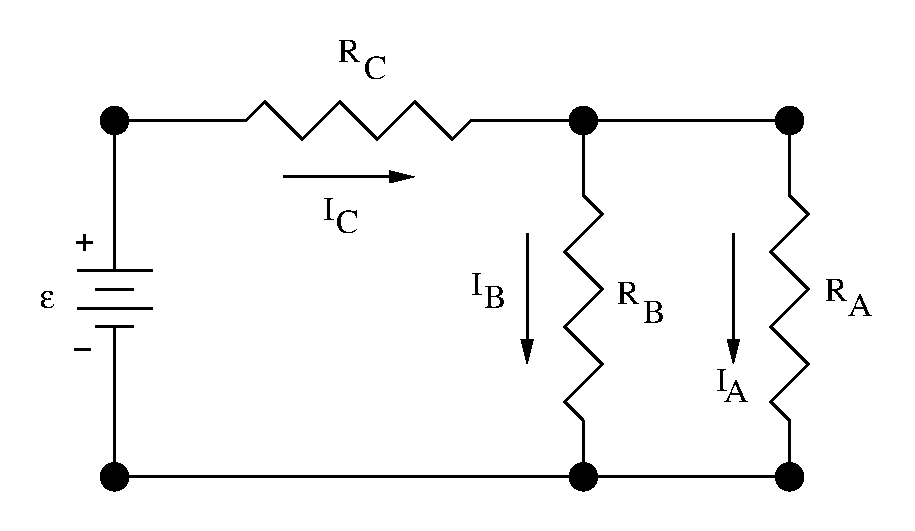
\includegraphics{kirchhoffs_rules/kirchhoffs_rules_fig_1.eps}} \par}
\vspace{0.3cm}

\begin{enumerate}[labparts]

\item Set one of your multimeters to resistance measuring mode. Remove $R_A$ from the circuit and measure its resistance with the multimeter and record the value below. Reconnect $R_A$ back to the circuit. Repeat this for $R_B$ and then for $R_C$.

\hspace{0.5in}$R_A=$

\hspace{0.5in}$R_B=$

\hspace{0.5in}$R_C=$


\item Referring to the circuit diagram above, choose a junction and write an equation
which satisfies Kirchhoff's first rule.
\answerspace{20mm}

\item Identify two closed loops on the circuit which contain at least one
element not included in the other. Write an equation for each loop
that satisfies Kirchhoff's second rule.
\answerspace{30mm}

\item You now have three equations that can be solved for the three currents $I_A$, $I_B$, and $I_C$.
Before doing the algebra, substitute the values of the three resistors that you determined in part~(a) into the loop equations. Further, substitute a value of 3.00~V for the emf. Carry out the algebra to obtain the values of the three currents.
\answerspace{5in}

\item Now use Ohm's law and the rules for combining resistors in series and parallel (i.e. reducing the circuit to equivalent circuits) to calculate the values of the three currents. Again use a value of 3.00~V for the emf and also use the values of the three resistors from your measurements.
\answerspace{3.5in}

\item Are the results of parts (d) and (e) the same? They should be.
\answerspace{15mm}

\item Make sure your circuit is complete and the power supply is still off. Connect one of your multimeters in parallel with the power supply in order to measure the voltage across the terminals of the power supply. Then, connect your second multimeter as an ammeter in series with $R_C$ in order to measure the current $I_C$. Now, turn the power supply on and adjust its output to read 3.00~V on the first multimeter. Record the value of $I_C$ below. Next, repeat the same procedure to measure similarly the currents $I_A$ and $I_B$. (Make sure the first multimeter still reads 3.00~V.) Record the values of the currents below.

\hspace{0.5in}$I_C =$

\hspace{0.5in}$I_A =$

\hspace{0.5in}$I_B =$

\bigskip
\item Do your results agree with those obtained in parts (d) and (e)? How large, in terms of percentage, are the discrepancies? Speculate on what might cause any differences. 

\answerspace{15mm}
\end{enumerate}

